\chapter{Funções}\label{cap:Funcoes}

\epigraph{``Nada que vale a pena é fácil''.}{Eric Cartman,  South Park}

\epigraph{``O ego é o pior inimigo do Eu, mas o Eu é o melhor amigo do ego... O ego é um péssimo senhor, mas é um ótimo servidor''.}{Bhagavad Gita}

\section{Conceitos, Definições e Nomenclaturas}\label{sec:FuncoesConceitoDefinicaoNomenclaturas}

Após o conceito importantíssimo de conjunto o componente mais importante na matemática é provavelmente a noção de função, o autor deste manuscrito não hesita em afirmar que você leitor com certeza já teve contato com a ideia de função, seja em seus curso do primário, secundário ou mesmo mais recentemente em suas disciplinas de nível superior tais como cálculo diferencial e integral ou alguma disciplina de física. 

Dado este encontra anterior do leitor sobre o assunto o autor fica confortável a pedir que leitor faça uma pequena pausa e tente lembrar de seus cursos anteriores e respondo para si mesmo ao questionamento: \textbf{o que é uma função}?

Bem, para muitos físicos, estatísticos e alguns matemáticos (não todos\footnote{Um visão interessante é aquela apontada em \cite{levin2021}, que descreve uma função como sendo um objeto com quatro descrições simultâneas: uma algébrica, uma numérica, uma gráfica e uma descritiva (ou em palavras).}), uma função é vista meramente como sendo um mapeamento (ou transformação) entre os elementos de dois conjuntos \cite{abe1991-TC}. Por outro lado, em obras tais como \cite{sussana2010-MD, lipschutz1971-Topo, lipschutz1978-TC, lipschutz2013-MD, Gerard2021discreta} uma função é vista como uma caso particular de relação entre dois conjuntos, ou seja, em última análise para esse grupo de pessoas uma função é exatamente um conjunto\footnote{Para melhor entender essa visão talvez o leitor deva revistar os Capítulos \ref{cap:Conjuntos} e \ref{cap:Relacoes} e revisar as definições apresentadas nos mesmo.}. Já em \cite{edward2019-MD, fmcbook} é apresentado uma visão mais mecanicista da ideia de função, essa visão captura a ideia de função enquanto uma máquina\footnote{Para cientistas da computação os termos máquina e programa são sinônimos.} (ou caixa preta) que transforma as entradas (\textit{inputs}) em saídas (\textit{outputs}), essa visão é ilustrada pela Figura \ref{fig:FuncaoBlackBox}. 

Há também a ideia de função como sendo uma estrutura \cite{judith2021}, com componentes bem estabelecidos. Essa visão é capaz (como será mostrado a seguir) de captura todas as outras ideias de função.  Neste manuscrito a formalização da ideia de função como sendo uma estrutura será apresentada de forma gradual trançando paralelos com as linguagens de programação que possuam um sistema de tipos, isso será adotado para tornar o texto mais didático e interessante ao leitor de computação, além disso, irá aproximar os tópicos teóricos (as funções) dos tópicos práticos (programação) cujo leitor desse manuscrito naturalmente tem contato e provável interesse. Entretanto, esse forma de apresentação não será menos rigorosa que outras fontes bibliográficas, na verdade será o oposto, o texto aqui apresentado tende a ser mais preciso e detalhado que a apresentação rasa feita em \cite{judith2021}, por exemplo.

\begin{figure}[h]
	\centering
	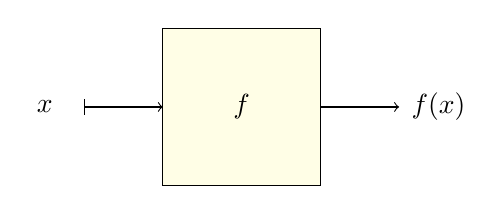
\begin{tikzpicture}
		\draw [rounded corners=0mm, fill=yellow!10]  (-1,1)--(-1,-1)--(1,-1)--(1,1)--cycle;
		\draw[->]  (1.0,0) -- (2.0,0.0);
	    \draw[|->]  (-2.0,0) -- (-1.0,0.0);
		\node (f) at (0,0) {$f$};
		\node (fx) at (2.5,0) {$f(x)$};
		\node (x) at (-2.5,0) {$x$};
	\end{tikzpicture}
	\caption{Visão de uma função de uma variável enquanto uma máquina (ou caixa preta).}
	\label{fig:FuncaoBlackBox}
\end{figure}

Este manuscrito irá iniciar o estudo sobre funções  apresentado ao leitor a ideia básica de assinatura de função, isto é, a seguir será apresentado a estrutura sintática que descreve as funções, ou seja, o componente descritivo mencionado em \cite{levin2021}.

\begin{definition}[Assinatura de Função]\label{def:AssinaturaFuncao}
	Sejam $A$ e $B$ conjuntos a assinatura da função de $A$ em $B$ nomeada como $f$ corresponde a uma palavra da forma $f: A \rightarrow B$.
\end{definition}

Note que a Definição \ref{def:AssinaturaFuncao} permite facilmente deduzir que em qualquer função existem três componentes básicos, sendo eles: um nome (rótulo ou símbolo funcional), um conjunto de partida e um conjunto de chegada. Por convenção, o nome de uma função deve ser sempre iniciado por caracteres latinos, no caso de usar índices apenas o último caractere do nome deve ser indexado.

\begin{example}\label{exe:AssinaturaFuncao}
	São exemplos de assinaturas de funções:
	\begin{itemize}
		\item[(a)] $g : \mathbb{N} \rightarrow \mathbb{Z}$.
		\item[(b)] $sqrt : \mathbb{R} \rightarrow \mathbb{R}$.
		\item[(c)] $k_1 : A \times B \rightarrow \mathbb{C}$.
		\item[(d)] $loc_2 : D \rightarrow \mathbb{R} \times \{0,1\}$.
		\item[(e)] $min : \mathbb{R}^n \rightarrow \mathbb{R}$.
		\item[(f)] $BUSCA : \mathbb{Z}^n \times \mathbb{Z} \rightarrow \{0,1\}$.
		\item[(g)] $BUSCA : \mathbb{R}^n \times \mathbb{R} \rightarrow \{0,1\}$.
	\end{itemize}
\end{example}

\begin{remark}
	O leitor deve observar que apesar das assinaturas nos itens (f) e (g) do Exemplo \ref{exe:AssinaturaFuncao} terem o mesmo nome, elas não são iguais, pois diferem no conjunto de partida, e assim não são a mesma assinatura. Esse tipo de cenário na computação recebe o nome de sobrecarga, isto é, o símbolo funcional $BUSCA$ está sobrecarregado para identificar duas funções distintas.
\end{remark}

Como dito anteriormente una função pode ser vista como uma máquina que transforma entradas em saídas, mas note que para que isso aconteça a máquina deve de alguma forma realizar ações sobre a entrada, ou seja, a máquina deve ``operar'' sobre a entrada. 

\begin{definition}[Aplicação]\label{def:Aplicacao}
	Seja $x_1, \cdots, x_n$ variáveis com $n \in \mathbb{N}_0$\footnote{Deste ponto em diante do manuscrito será considerado $\mathbb{N}_0 = \mathbb{N} - \{0\}.$} e $E$ uma palavra válida, a aplicação das variáveis $x_1, \cdots, x_n$ sobre a palavra $E$, é denotado por  $x_1, \cdots, x_n \mapsto E$, onde $E$ é uma palavra válida em algum contexto formal\footnote{No contexto da matemática, por exemplo, a palavra $x + (2\sqrt{14} - 3)$ é válida e a palavra $(\frac{1}{\log +})\sqrt{5}$ não é válida.}.
\end{definition}

Note que a Definição \ref{def:Aplicacao} apenas descreve que as entradas (as variáveis) devem ser aplicada sobre a palavra $E$, assim uma aplicação no sentido como se está apresentado não se preocupa com o tipo das variáveis ou o tipo da palavra de saída. Por exemplo, imagine a aplicação $x \mapsto 2x + 1$, tal aplicação diz que a variável de entrada $x$ gera a palavra de saída $2x + 1$. Assim a noção de aplicação como definida anteriormente se assemelha a noção de $\lambda$-termo (para detalhes vê \cite{bare1984, bimbo2019, hankin2004}) em uma teoria de $\lambda$-cálculo não tipado \cite{henk1992, hankin2004}, ou seja, a aplicação em si está definido uma função sem nomear ou tipar os argumentos de entrada da mesma, o $\lambda$-cálculo em si será trato mais adiante neste manuscrito.

\begin{example}\label{exe:Aplicacoes}
	São exemplos de aplicações:
	\begin{itemize}
		\item[(a)] $x \mapsto log_2 x$.
		\item[(b)] $x, y \mapsto 3^x + x$.
		\item[(c)] $x, y, z \mapsto 4$.
		\item[(d)] $x, y, z \mapsto \sqrt[z]{\frac{1}{2}x + y}$.
	\end{itemize}
\end{example}

\begin{remark}
	Os itens (b), (c) e (d) do Exemplo \ref{exe:Aplicacoes} permitem concluir que em uma aplicação as variáveis de entrada, isto é, os símbolos à esquerda de $\mapsto$, podem aparecer de forma integral, parcial e nem aparecer na palavra de saída $E$ à direita de $\mapsto$.    
\end{remark}

Note que uma aplicação expressa a ação que deve ser feita em relação as variáveis de entrada, assim a semântica de uma aplicação  $x \mapsto x + 1$ é: Dado um $x$ construa e devolva\footnote{Aqui devolva é no resultado de retorna o que foi construído como resultado da aplicação.} $x + 1$. Agora observe que até o presente momento aplicação foi tratada de forma genérica, isto é, são utilizadas variáveis para gerar a palavra de saída. Mas uma vez que a entrada são variáveis, significa que as mesma podem ser substituídas (possivelmente) por infinitos valores, gerando assim infinitas palavras, uma para cada entrada. Esta ação de substituir as variáveis por elementos específicos, isto é, símbolos constantes específicos, será chamada de \textbf{uso} da aplicação, sendo formalizado a seguir.

\begin{definition}[Uso de uma aplicação]\label{def:UsoAplicacao}
	O uso da aplicação $x_1, \cdots, x_n \mapsto E$ para as palavras $y_1, \cdots, y_n$, denotado por $(x_1, \cdots, x_n \mapsto E)y_1, \cdots, y_n$, corresponde ao ato de substituir em $E$ toda referência de $x_i$ por $y_i$ com $1 \leq i \leq n$.
\end{definition}

\begin{example}\label{exe:UsoAplicacao}
	São exemplos de usado de aplicações:
	\begin{itemize}
		\item[(a)] Considerando $x \mapsto x + 1$ tem-se que $(x \mapsto x + 1)3$ gera a palavra $3 + 1$, e $(x \mapsto x + 1)10$ gera a palavra $10 + 1$.
		\item[(b)] Dado $x, y \mapsto 3^x + x$ tem-se que $(x, y \mapsto 3^x + x)4,5$ gera a palavra $3^4 + 4$. Além disso,  tem-se que $(x, y \mapsto 3^x + x)4,5,1$ não é um uso válido, pois a aplicação só possui duas variáveis, mas o uso tenta usar a aplicação para três valores.
		\item[(c)] Considerando $x, y, z \mapsto 14$ tem-se que $(x, y, z \mapsto 14)1, 2, 3$ gera a palavra $14$, e $(x, y, z \mapsto 14)3, 1, 3$ também gera a palavra $14$.
	\end{itemize}
\end{example}

Para o leitor experiente pode notar que a noção de uso da aplicação nada mais é do que a noção de $\beta$-redução existente em $\lambda$-cálculo \cite{bare1984}. 

\begin{remark}\label{rema:ReducaoFuncao}
	Para evitar ficar escrevendo que $(x_1, \cdots, x_n \mapsto E)y_1, \cdots, y_n$ gera uma palavra $E'$, é possível escrever $(x_1, \cdots, x_n \mapsto E)y_1, \cdots, y_n \rightsquigarrow E'$.
\end{remark}

Agora é comum em matemática como dito em \cite{carmo2013}, após o uso de uma aplicação verificar se existem símbolos que podem ser interpretados como operações, caso existam os mesmos devem ser usado afim de ser gerada a menor palavra (em número de símbolos) possível.

\begin{example}
	Dado as mesma aplicações e usos dos itens (a) e (b) Exemplo \ref{exe:UsoAplicacao} tem-se que $(x \mapsto x + 1)3 \rightsquigarrow 4$, $(x \mapsto x + 1)10 \rightsquigarrow 11$ e $(x, y \mapsto 3^x + x)4,5 \rightsquigarrow 85$.
\end{example}

\begin{example}
	Dado a aplicação $x \mapsto -2x$ tem-se que $(x \mapsto -2x)-4 \rightsquigarrow -8$.
\end{example}

\begin{definition}[Igualdade de uso]\label{def:IgualdadeUsoAplicacoes}
	Dado $x_1, \cdots, x_n \mapsto E$, $y_1, \cdots, y_n$ e $z_1, \cdots, z_n$, o uso de aplicação  $x_1, \cdots, x_n \mapsto E$ para $y_1, \cdots, y_n$ é igual ao uso para $z_1, \cdots, z_n$, denotado pela igualdade usual $(x_1, \cdots, x_n \mapsto E)y_1, \cdots, y_n = (x_1, \cdots, x_n \mapsto E)z_1, \cdots, z_n$, sempre que: $(x_1, \cdots, x_n \mapsto E)y_1, \cdots, y_n \rightsquigarrow E'$ e  $(x_1, \cdots, x_n \mapsto E)z_1, \cdots, z_n \rightsquigarrow E'$, onde $E'$ é uma palavra irredutível.
\end{definition}

\begin{example}
	Dado a aplicação $x, y \mapsto \frac{(x+y)}{2}$ tem-se que $(x, y \mapsto \frac{(x+y)}{2})2, 4 \rightsquigarrow 3$ e  $(x, y \mapsto \frac{(x+y)}{2})3, 3 \rightsquigarrow 3$, logo pode-se escrever que $(x, y \mapsto \frac{(x+y)}{2})2, 4 = (x, y \mapsto \frac{(x+y)}{2})3, 3$. Por outro lado, $(x, y \mapsto \frac{(x+y)}{2})6, 12 \rightsquigarrow 9$ e, assim, $(x, y \mapsto \frac{(x+y)}{2})2, 4 \neq (x, y \mapsto \frac{(x+y)}{2})6, 12$
\end{example}

\begin{proposition}
	Dado $x_1, \cdots, x_n \mapsto E$ e $y_1, \cdots, y_n$ e $z_1, \cdots, z_n$. Se existe $1 \leq i \leq n$ tal que $y_i \neq z_i$, então $(x_1, \cdots, x_n \mapsto E)y_1, \cdots, y_n \neq (x_1, \cdots, x_n \mapsto E)z_1, \cdots, z_n$.
\end{proposition}

\begin{proof}
	Direto das definições \ref{def:UsoAplicacao} e \ref{def:IgualdadeUsoAplicacoes}.
\end{proof}


Agora que foram apresentados estes conceitos fundamentais pode-se continuar o desenvolvimento deste texto com a formalização da ideia de função.

\begin{definition}[Função]
	Dado uma assinatura $f: A \rightarrow B$ e seja $x \mapsto E$ uma aplicação, a estrutura da forma $\langle f: A \rightarrow B, x \mapsto E \rangle$ é uma função sempre que para todo $e \in A$ se $(x \mapsto E)e \rightsquigarrow E'$, então $E' \in B$.
\end{definition}

% Susam, lipstick (topo),  ver como relação